\documentclass[10pt]{scrartcl} 

\usepackage[a4paper,left=1.5cm,right=1.5cm,top=2cm,bottom=2cm,bindingoffset=5mm]{geometry}

%% allgemeine Imports, die nicht mehr erforderlich sind, da ich mit lulatex kompiliere
% \usepackage[utf8x]{inputenc} % Zeichenkodierung
% \usepackage[ngerman]{babel}  % u.a. Silbentrennung
% \usepackage[T1]{fontenc}

%\usepackage{floatflt} 
%\usepackage{times}

%\usepackage{amsmath} %Bei Bedarf: Formeln
\usepackage{graphicx}   % Bilder
\graphicspath{{./image/}{./plantuml/}{./}}
%\begin{figure}[htbp] 
%	\centering
%	\includegraphics[width=3cm]{JavaSpringInitializr.png}
%	\caption{Logo}
%	\label{fig:Bild1}
%\end{figure}



\usepackage{wrapfig}
%\begin{wrapfigure}{l}{0.25\textwidth}
%	\centering
%	\includegraphics[width=0.25\textwidth]{contour}
%\end{wrapfigure}

\usepackage{lastpage} %Letzte Seitenzahl anzeigen
\usepackage{hyperref}
\usepackage{cclicenses}

%\usepackage{blindtext}  %% Zum Debugging: Blindtext einfügen

%%% zur Darstellung von Quellcode
\usepackage{listings}
\usepackage{color}
\usepackage{xcolor}

%%% Für individuelle Kopfzeilen
% https://esc-now.de/_/latex-individuelle-kopf--und-fusszeilen/?lang=en
%%%%%%%%%%%%%%%%%%%%%%%%%%%
\usepackage[headsepline=0.5pt,footsepline=0.5pt,plainheadsepline=true, plainfootsepline=true,headwidth=(\the\textwidth), footwidth=(\the\textwidth)]{scrlayer-scrpage}

% Alle Inhalte löschen.
\clearpairofpagestyles

%\renewcommand{\familydefault}{\sfdefault}

% Schriftformatierung zurücksetzen.
\setkomafont{pageheadfoot}{}
\setkomafont{title}{\bfseries}

% Linien einfärben.
\addtokomafont{headsepline}{\color{gray}}
\addtokomafont{footsepline}{\color{gray}}

% Statische Inhalte.
\ihead{\thetitle}
%\chead{Mitte oben}
\ohead{
	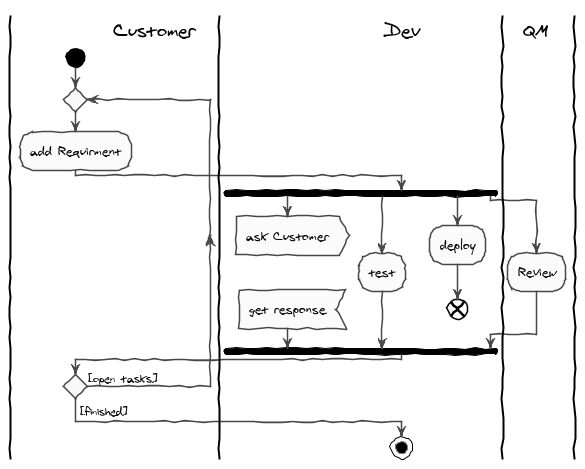
\includegraphics[height=1cm]{logo}	
}


% Unterschiedliche Inhalte für gerade/ungerade.
\ifoot*{\href{https://creativecommons.org/licenses/by/4.0/}{\ccby CC BY 4.0}, Hannes Stein  }
\cfoot*{\today}
\ofoot*{\pagemark}
\renewcommand*{\pagemark}{{\usekomafont{pagenumber}{Seite \thepage\ von \pageref*{LastPage}}}}


%\usepackage{showframe} % for debug information
\usepackage{titling}
\pretitle{
	
\begin{tabular}[b]{p{11cm} p{5cm}}
      \bfseries
		\LARGE
		\selectfont
		}
\posttitle{
 & 	
 \raisebox{-\height}{
 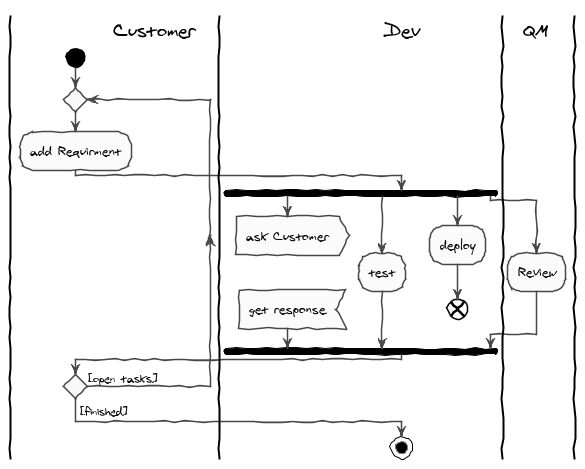
\includegraphics[width=4.5cm]{logo}
}
	\end{tabular}
}
%\preauthor{}\postauthor{}
\predate{}\date{}\postdate{}


%%%%%%%%%%%%%%%%%%%%%%%%%


%%% zur Darstellung von Quellcode
\definecolor{dkgreen}{rgb}{0,0.6,0}
\definecolor{gray}{rgb}{0.5,0.5,0.5}
\definecolor{lightgray}{rgb}{0.83, 0.83, 0.83}
\definecolor{mauve}{rgb}{0.58,0,0.82}

\lstset{
	frame=tb,	
	aboveskip=3mm,
	belowskip=3mm,
	columns=fixed,
	basicstyle={\small\ttfamily},
	numbers=left,
	numberstyle=\tiny\color{gray},
	firstnumber=last,
	keywordstyle=\color{blue},
	commentstyle=\color{dkgreen},
	stringstyle=\color{mauve},
	breaklines=true,
	breakatwhitespace=true,
	tabsize=3,
	includerangemarker=true,
	showtabs=false,
	showspaces=false
}

\lstdefinestyle{java}{
	language=Java,
	numbers=left, stepnumber=1, numberstyle=\tiny, numbersep=10pt}
\lstdefinestyle{bashquery}{
	language=bash,
	numbers=left,
	stepnumber=1,
	numberstyle=\tiny,
	numbersep=10pt}
\lstdefinestyle{response}{
	frame=trbl,
	aboveskip=0mm,
	belowskip=3mm,
	basicstyle={\scriptsize\ttfamily},
	frame=shadowbox, 
	rulecolor=\color{lightgray},
	rulesepcolor=\color{lightgray},
	numbers=none
}

\lstdefinestyle{nonumbers}{
	numbers=none
}

\lstdefinestyle{plantuml}{
	numbers=left, stepnumber=1, numberstyle=\tiny, numbersep=10pt,
	morekeywords=[1]{actor, usecase, rectangle, as},
	morekeywords=[2]{skinparam, ArrowColor, BorderColor, BackgroundColor},
	morekeywords=[3]{DefaultFontName},
	morekeywords=[4]{whitesmoke, DarkSlateBlue, LightYellow},
	morekeywords=[5]{note, top, on, link, end, left to right, direction, up, down, left, right},
	morekeywords=[6]{start, stop, @startuml, @enduml, if(), if, then, else, endif, elseif, repeat, while, is },
	morekeywords=[7]{endwhile},
	morekeywords=[8]{:,  .., .,  -, --, ->, -->, -|>, --|>, <-, <--, <|-, <|--, <., <.., <|., <|.., \\n, \{, \}, ;},
	morecomment=[l]{'}
	}


%\hypersetup{
%	pdftitle    = { hihihi },
%	pdfsubject  = {Um was geht es },
%	pdfauthor   = {Autor bzw. Autoren},
%	pdfkeywords = {Stichwort1, Stichwort2 ...} ,
%	baseurl = {http://www.csbme.de},
%	pdfdisplaydoctitle = true
%}


\title{UML Aktivitätsdiagramm\\
	und die Modellierung mit plantUML
 }
%\author{Hannes Stein}





\begin{document}
	\setlength{\droptitle}{-40pt} % lower the title
	\maketitle
%	\begin{abstract}
%	Wie interagiert ein (Software-)System mit dem Benutzer?
%	\end{abstract}

	

%\pagenumbering{roman}\setcounter{page}{1}
% \tableofcontents
% \listoffigures
% \listoftables



\pagenumbering{arabic}\setcounter{page}{1}

\section{Diagramm zur Verhaltensmodellierung}
Ein UML-Aktivitätsdiagramm (\textit{Activitydiagram}) beschreibt, wie das Verhalten eines (Software)-System \textit{realisiert} ist. Es erweitert die Ausdrucksmöglichkeiten gegenüber einfacheren Flussdiagrammen wie dem Programmablaufplan. Im Aktivitätsdiagramm können Daten- und Kontrollflüsse modelliert werden, z.B. von

\begin{itemize}
	\item Algorithmen,
	\item Geschäftsprozessen oder
	\item Workflows.
\end{itemize}
Im Fokus steht die Modellierung der Abfolge (sequenziell oder parallel), Bedingungen, Verzweigungen, Wiederholungen sowie Anfang und Ende von Aktivitäten. Alle Schritte können zudem in Verantwortungsbereichen konkreten Akteurinnen oder Systemen zugewiesen werden.
\section{Das Tokenmodell im Flussdiagramm: mit Knoten und Kanten}

\begin{tabular}[b]{p{10cm} p{7cm}}
Aktivitätsdiagramme bestehen aus \textbf{Knoten} und \textbf{Kanten}. Sie nutzen das Tokenmodell: ein \textit{Token} ist eine gedachte Markierung (\textit{Token}) kennzeichnet die momentan ausgeführten Aktionen - vergleichbar mit dem springenden Punkt beim Karaokesingen. Ein Token wird im Startpunkt (\textit{initial node}) erzeugt und durchläuft das Diagramm entlang der Kanten (Pfeile, \textit{edges}). Im Endpunkt (\textit{activity final node}) wird der Token konsumiert und die Aktivität so beendet.

Ein minimales mit PlantUML modelliertes Aktivitätsdiagramm, das einen unverzweigte Aktivität darstellt, ist rechts dargestellt.

	&
	
	\raisebox{-\height}{
	\href{http://www.plantuml.com/plantuml/proxy?fmt=svg&src=https://raw.githubusercontent.com/hannsens/plantUML-Activity-Infosheet/master/plantuml/01_aktion_start_stop.plantuml}{
	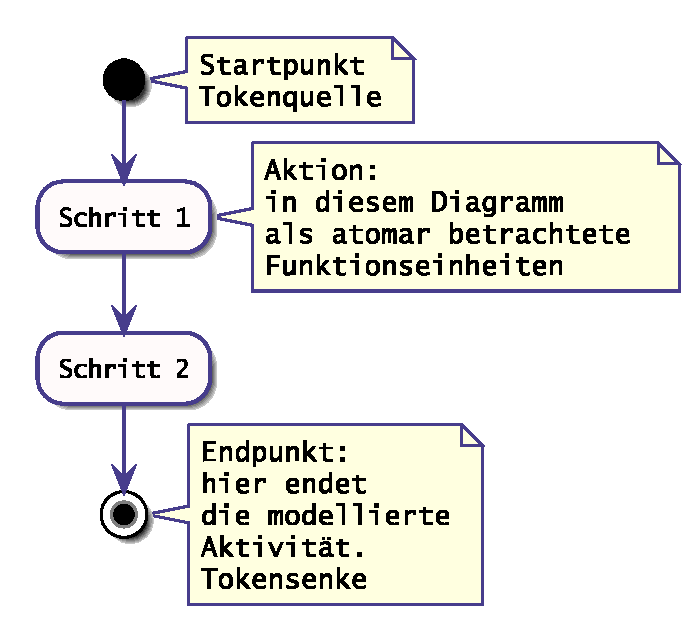
\includegraphics[width=6.5cm]{01_aktion_start_stop}
}
}
\end{tabular}
Hinweis: Den meisten Diagrammen in diesem Dokument sind Links zu den zugrundeliegenden Vektorgrafiken und Quelltexten hinterlegt. Der die komplette URL öffnet das Diagramm, die zweite Hälfte (nach src=) den Quelltext.

\href{http://www.plantuml.com/plantuml/proxy?fmt=svg&src=https://raw.githubusercontent.com/hannsens/plantUML-Activity-Infosheet/master/plantuml/01_aktion_start_stop.plantuml}{https://www.plantuml.com/plantuml/proxy?fmt=svg\&src=https://www.quelltext.url/source.plantuml}

\begin{tabular}[b]{p{7cm} p{10cm}}
	
	\raisebox{-\height}{
		\href{http://www.plantuml.com/plantuml/proxy?fmt=svg&src=https://raw.githubusercontent.com/hannsens/plantUML-Activity-Infosheet/master/plantuml/02_minimalbeispiel.plantuml}{
		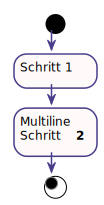
\includegraphics[width=2cm]{02_minimalbeispiel}
	}
	}
	&
	\begin{lstlisting}[style=plantuml]
@startuml 'Muss immer am Anfang stehen
start
:Schritt 1;
:Multiline
	Schritt **2**;
stop
@enduml
	\end{lstlisting}
\end{tabular}


\newpage
\section{Kontrollstrukturen: Verzweigung und Vereinigung}
Neben dem rein sequenziellen unverzweigten Ablauf können auch bedingte Anweisungen modelliert werden. Verzweigungen werden als Entscheidungsknoten (\textit{decision node}) mit dem Raute-Symbol notiert. Die Bedingungen selbst werden als \textit{guard} bezeichnet und -abweichend vom Programmablaufplan- in eckigen Klammern an der jeweiligen Kante notiert. Die Bedingungen müssen als Prädikat formuliert sein - also mit \textit{true} oder \textit{false} auswertbar sein. Sie sollten \textit{disjunkt} sein (sich gegenseitig ausschließen), um ein vorhersagbares Verhalten zu modellieren. Bei einfachen Verzweigungen erreicht man das, in dem zu jeder Bedingung ein \texttt{[else]}-Zweig modelliert wird.

\begin{tabular}[b]{p{7cm} p{10cm}}
	
	\raisebox{-\height}{
		\href{http://www.plantuml.com/plantuml/proxy?fmt=svg&src=https://raw.githubusercontent.com/hannsens/plantUML-Activity-Infosheet/master/plantuml/03_einfacheBedingung.plantuml}{
		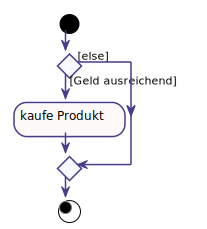
\includegraphics[width=4cm]{03_einfacheBedingung}
	}
	}
	&
	Bei PlantUML ist die Notation etwas gewöhnungsbedürftig: die erste Bedingung wird hinter \texttt{then()} in Klammern notiert, den \texttt{else}-Block sollte man in jedem Fall notieren:
	\begin{lstlisting}[style=plantuml]
if() then ([Geld ausreichend])
	:kaufe Produkt;
else ([else])
endif
	\end{lstlisting}
	Im Gegensatz zum Programmablaufplan werden die verschiedenen Kanten einer Verzweigung auch wieder an einer Raute (\textit{merge node}) zusammengeführt. Weder ein \textit{decision node} noch ein \textit{merge node} ändern die Anzahl der vorhandenen Token.
\end{tabular}


\begin{tabular}[b]{p{7cm} p{10cm}}
	
	\raisebox{-\height}{
		\href{http://www.plantuml.com/plantuml/proxy?fmt=svg&src=https://raw.githubusercontent.com/hannsens/plantUML-Activity-Infosheet/master/plantuml/03_einfacheVerzweigung.plantuml}{
		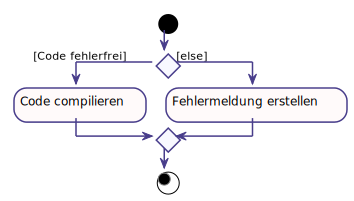
\includegraphics[width=6.5cm]{03_einfacheVerzweigung}
		}
	}
	&
	
	\begin{lstlisting}[style=plantuml]
start
if() then ([Code fehlerfrei])
	:Code compilieren;
else ([else])
	:Fehlermeldung erstellen;
endif
stop
	\end{lstlisting}
\end{tabular}


Nicht alle Bedingungen lassen sich unmittelbar als Prädikat formulieren. Sofern nähere Eräuterungen nötig sind sieht die UML vor, dass diese über eine Notiz mit dem Stereotyp \texttt{<<decision input>>} erfolgt, die mit der \textit{decision node} verbunden wird.

In PlantUML gibt es diese Möglichkeit nicht, daher muss man sich mit einer Notiz, die neben der vorigen Aktion steht, behelfen. Gemäß UML wird innerhalb der \textit{decision node} nichts notiert - hier weicht die PlantUML-Dokumentation vom UML-Standard ab.

\begin{tabular}[b]{p{7cm} p{10cm}}
	\raisebox{-\height}{
		\href{http://www.plantuml.com/plantuml/proxy?fmt=svg&src=https://raw.githubusercontent.com/hannsens/plantUML-Activity-Infosheet/master/plantuml/03_komplexereVerzweigung.plantuml}{
		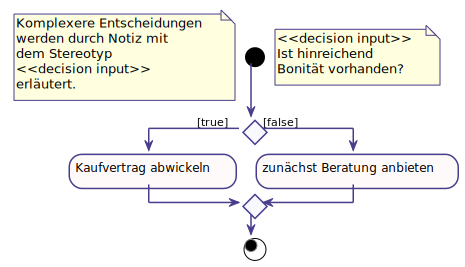
\includegraphics[width=6.5cm]{03_komplexereVerzweigung}
		}
	}
	&
	\begin{lstlisting}[style=plantuml]
note right
	<<decision input>>
	Ist hinreichend 
	Bonität vorhanden?
end note
if() then ([true])
	:Kaufvertrag abwickeln;
else ([false])
	:zunächst Beratung anbieten;
endif
	\end{lstlisting}
\end{tabular}
\newpage
Mehrfache Verzweigungen können durch mehr Kanten realisiert werden, die den \textit{decision node} verlassen. Wichtig ist auch hier, dass die \textit{guards} disjunkt sind.

Leider bietet PlantUML nur die Möglichkeit, zwei ausgehende Kanten an einer \textit{decision node} zu nutzen. Daher müssen multiple Bedingungen als verschachtelte If-Statements modelliert werden:

\begin{tabular}[b]{p{7cm} p{10cm}}
	
	\raisebox{-\height}{
		\href{http://www.plantuml.com/plantuml/proxy?fmt=svg&src=https://raw.githubusercontent.com/hannsens/plantUML-Activity-Infosheet/master/plantuml/03_mehrfacheVerzweigung.plantuml}{
		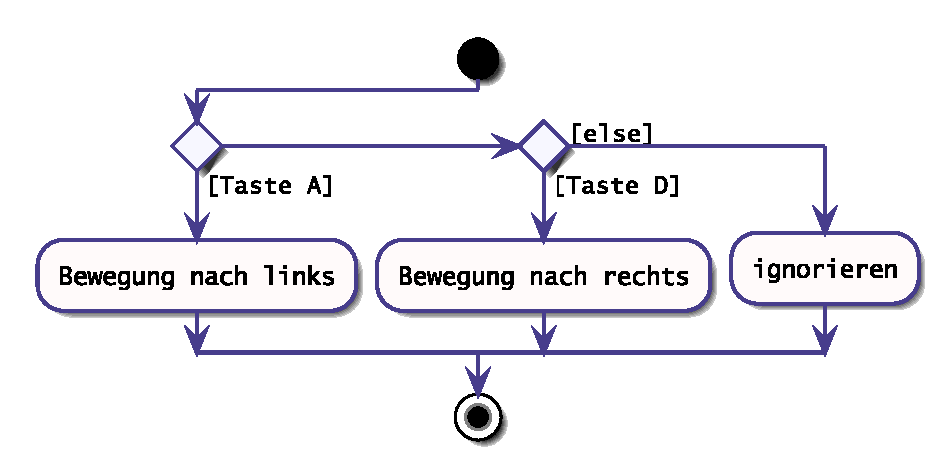
\includegraphics[width=6.5cm]{03_mehrfacheVerzweigung}
		}
	}
	&
	
	\begin{lstlisting}[style=plantuml]
if() then ([Taste A])
	:Bewegung nach links;
elseif() then ([Taste D])
	:Bewegung nach rechts;
else ([else])
	:ignorieren;
endif
	\end{lstlisting}
\end{tabular}

\section{Wiederholungsstrukturen: kopf- und fussgesteuerte Schleifen}
Eine nachgelagerte Bedingung, die eine Wiederholung bestimmter Aktionen erzwingt wird über die Rückführung der ausgehenden Kante mit \textit{guard} einer \textit{decision node} modelliert. Bei diesen fussgesteuerten Schleifen werden die Aktionen innerhalb der Schleife in jedem Fall einmal ausgeführt. Mit PlantUML erfolgt die Modellierung mit einem \texttt{repeat / repeat while () is ([ }\textit{guard} \texttt{])}-Block:

\begin{tabular}[b]{p{7cm} p{10cm}}
	
	\raisebox{-\height}{
		\href{http://www.plantuml.com/plantuml/proxy?fmt=svg&src=https://raw.githubusercontent.com/hannsens/plantUML-Activity-Infosheet/master/plantuml/04_fussgesteuerteSchleife.plantuml}{
		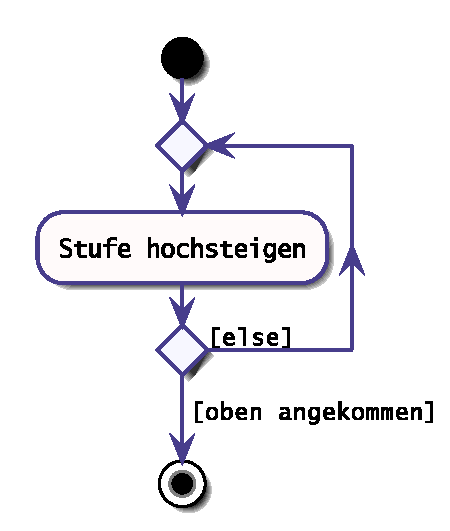
\includegraphics[width=4cm]{04_fussgesteuerteSchleife}
		}
	}
	&
	
	\begin{lstlisting}[style=plantuml]
start
repeat
	:Stufe hochsteigen;
repeat while () is ([else])
->[oben angekommen];
stop


	\end{lstlisting}
\end{tabular}

Im Fall einer kopfgesteuerten Schleife wird die Bedingung zunächst geprüft, die zu wiederholenden Aktionen also ggf. nie ausgeführt.

\begin{tabular}[b]{p{7cm} p{10cm}}
	
	\raisebox{-\height}{
		\href{http://www.plantuml.com/plantuml/proxy?fmt=svg&src=https://raw.githubusercontent.com/hannsens/plantUML-Activity-Infosheet/master/plantuml/04_kopfgesteuerteSchleife.plantuml}{
		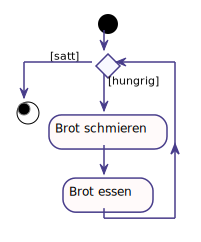
\includegraphics[width=4cm]{04_kopfgesteuerteSchleife}
		}
	}
	&
	
	\begin{lstlisting}[style=plantuml]
start
while() is ([hungrig])
	:Brot schmieren;
	:Brot essen;
endwhile ([satt])
stop

	\end{lstlisting}
\end{tabular}
\newpage
\section{Concurrency: Parallelisierung von Aktionen (Splitting und Synchronisation)}
Im Gegensatz zu einem \textit{decision node} oder \textit{merge node} müssen bei Gabelungen (\textit{fork node}) oder Synchronisierung (\textit{join node}) an allen eingehenden Kanten ein Token anliegen, damit sie wiederum Token weiterreichen. Entsprechend werden an allen ausgehenden Kanten dann Token weitergereicht. Auf diese Art werden parallele Prozesse und Synchronisierungen modelliert.

\begin{tabular}[b]{p{7cm} p{10cm}}
	
	\raisebox{-\height}{
		\href{http://www.plantuml.com/plantuml/proxy?fmt=svg&src=https://raw.githubusercontent.com/hannsens/plantUML-Activity-Infosheet/master/plantuml/05_concurrency.plantuml}{
		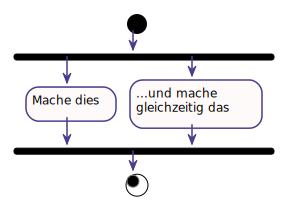
\includegraphics[width=6cm]{05_concurrency}
		}
	}
	&
	
	\begin{lstlisting}[style=plantuml]
start
fork
	:Mache dies;
fork again
	:...und mache 
	gleichzeitig das;
end fork
stop

	
	\end{lstlisting}
\end{tabular}


\section{Partitionen / Swimlanes zur Unterscheidung von Verantwortungsbereichen}
Die UML sieht vor, dass modelliert werden kann, welche Akteurin oder welches System für bestimmte Aktionen verantwortlich oder organisatorisch Zuständig ist. Aufgrund des Aussehens werden diese Verantwortungsbereiche, die die UML \textit{partition} nennt, oft \textit{swimlanes} genannt.

\begin{tabular}[b]{p{7cm} p{10cm}}
	
	\raisebox{-\height}{
		\href{http://www.plantuml.com/plantuml/proxy?fmt=svg&src=https://raw.githubusercontent.com/hannsens/plantUML-Activity-Infosheet/master/plantuml/06_swimlanes.plantuml}{
		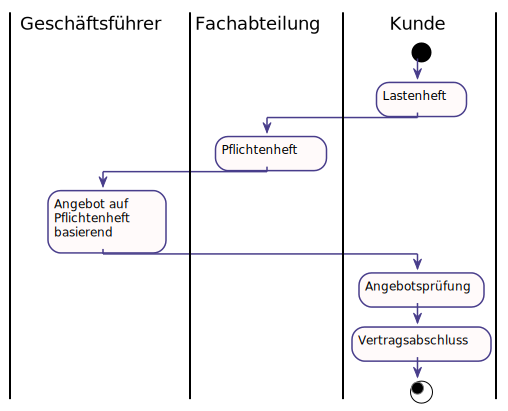
\includegraphics[width=6.5cm]{06_swimlanes}
		}
	}
	&
	
	\begin{lstlisting}[style=plantuml]
'Durch Nennung Reihenfolge festlegen
|Geschäftsführer|
|Fachabteilung|
|Kunde|
	start
|Kunde|
	:Lastenheft;
|Fachabteilung|
	:Pflichtenheft;
|Geschäftsführer|
	:Angebot auf 
	Pflichtenheft 
	basierend;
|Kunde|
	:Angebotsprüfung;
	:Vertragsabschluss;
	stop
\end{lstlisting}
\end{tabular}

\section{Signale/ Ereignisse senden und empfangen; Objektflüsse darstellen}

Token können nicht nur aus einem Startknoten entspringen, sondern auch über Signale erzeugt werden, die in einer \textit{accept event action} empfangen werden. Sofern dieser Signalempfängerknoten auch eingehende Kanten hat, wird der ausgehende Token erst gefeuert, wenn ein Token anliegt und ein Signal eingeht. Der Token wandert dann wie gewohnt entlang der Kanten von Knoten zu Knoten. 
Signale können auch gesendet werden. Beim erreichen einer \textit{send signal action} wird asynchron das Signal gesendet und die nächste Aktion bearbeitet. Es wird nicht auf Antwort oder Empfangsbestätigung gewartet.

Sofern nicht der Kontrollfluss symbolisiert werden soll, sondern konkrete Daten, so wird ein Objektknoten als Rechteck notiert. An den ein- und ausgehenden Kanten wird anstelle eines abstrakten Tokens dann ein Objekt transportiert.

\begin{tabular}[b]{p{7cm} p{10cm}}
	
	\raisebox{-\height}{
		\href{http://www.plantuml.com/plantuml/proxy?fmt=svg&src=https://raw.githubusercontent.com/hannsens/plantUML-Activity-Infosheet/master/plantuml/07_signals.plantuml}{
		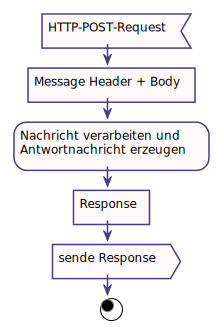
\includegraphics[width=4cm]{07_signals}
		}
	}
	&
	
	\begin{lstlisting}[style=plantuml]
	
:HTTP-POST-Request<
:Message Header + Body]
:Nachricht verarbeiten und 
	Antwortnachricht erzeugen;
:Response]
:sende Response>
stop
	\end{lstlisting}
\end{tabular}

\section{Ablaufende}
Wenn das Erreichen eines Endes zwar den aktuellen Ausführungsstrang beendet - also den eingetroffenen Token konsumiert - aber in der Gesamtaktivität noch weitere Token vorhanden sein können, muss ein Ablaufende ()\textit{activity final node}) modelliert werden.
Im Gegensatz zu einem \textit{activity final node} werden nicht alle vorhandenen Token konsumiert, sondern nur der am \textit{activity final node} eintreffende Token.

\begin{tabular}[b]{p{7cm} p{10cm}}
	
	\raisebox{-\height}{
		\href{http://www.plantuml.com/plantuml/proxy?fmt=svg&src=https://raw.githubusercontent.com/hannsens/plantUML-Activity-Infosheet/master/plantuml/08_ablaufende.plantuml}{
		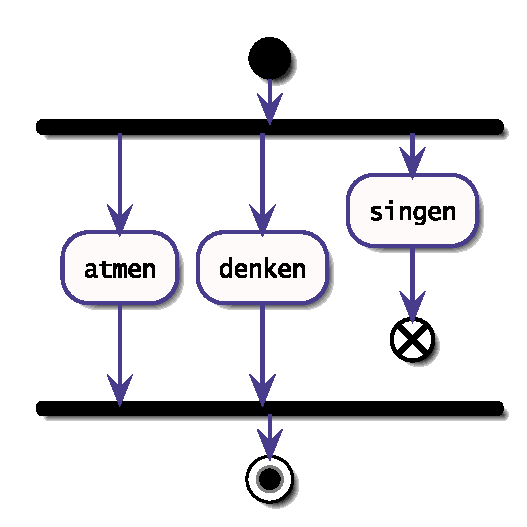
\includegraphics[width=4cm]{08_ablaufende}
		}
	}
	&
	
	\begin{lstlisting}[style=plantuml]
start
fork
	:atmen;
fork again
	:denken;
fork again
	:singen;
	end
end fork
stop
	\end{lstlisting}
\end{tabular}


\section{Konnektoren (Sprungmarken) zur übersichtlicheren Darstellung}
Um Kreuzungen zu vermeiden oder um komplexere Zusammenhänge übersichtlicher darstellen zu können, können Sprungmarken (A) verwendet werden. Abläufe können dadurch unterbrochen werden (bei PlantUML mit \texttt{detach}) und in gesonderten Aktivitätsdiagrammen ausgeführt werden.

\begin{tabular}[b]{p{7cm} p{10cm}}
	
	\raisebox{-\height}{
		\href{http://www.plantuml.com/plantuml/proxy?fmt=svg&src=https://raw.githubusercontent.com/hannsens/plantUML-Activity-Infosheet/master/plantuml/09_sprungmarke.plantuml}{
		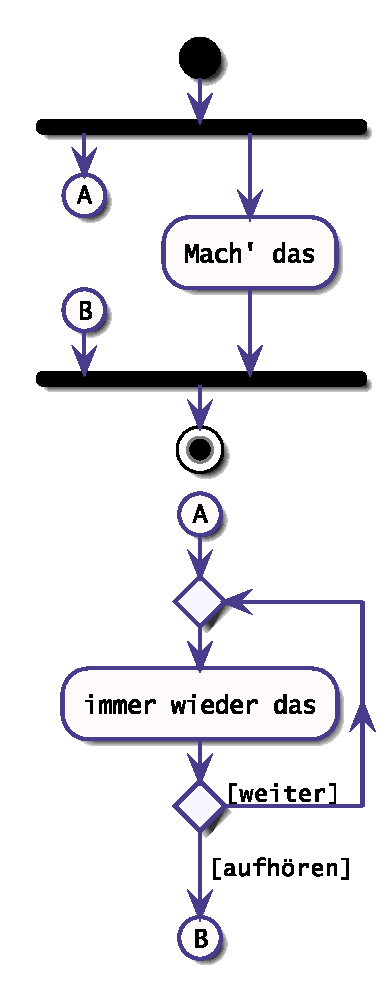
\includegraphics[width=3cm]{09_sprungmarken}
		}
	}
	&
	
	\begin{lstlisting}[style=plantuml]
start
fork
	(A)
	detach
	(B)
fork again
	:Mach' das;
end fork 
stop


(A)
repeat
	:immer wieder das;
repeat while () is ([weiter])
->[aufhören];
(B)

	\end{lstlisting}
\end{tabular}


\section{Vor- und Nachbedingungen}
Aktionen können mit Vor- und Nachbedingungen versehen werden. Diese werden jeweils als Notiz mit dem jeweiligen Stereotyp notiert:
\begin{itemize}
	\item <<localPrecondition>>: Diese Bedingungen müssen vor Eintritt in die Aktion erfüllt sein
\item <<localPostcondition>> : Diese Bedingungen müssen vor Beendigung der Aktion erfüllt sein
\end{itemize}

\begin{tabular}[b]{p{7cm} p{10cm}}
	
	\raisebox{-\height}{
		\href{http://www.plantuml.com/plantuml/proxy?fmt=svg&src=https://raw.githubusercontent.com/hannsens/plantUML-Activity-Infosheet/master/plantuml/10_vornachbedingung.plantuml}{
		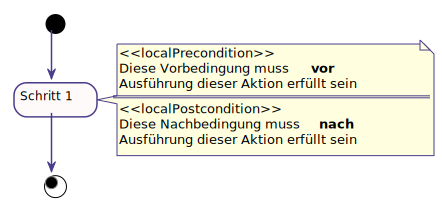
\includegraphics[width=6.5cm]{10_vornachbedingung}
		}
	}
	&
	
	\begin{lstlisting}[style=plantuml]
start
:Schritt 1; 
note right 
	<<localPrecondition>>
	Diese Vorbedingung muss <b>vor</b> 
	Ausführung dieser Aktion erfüllt sein
	====
	<<localPostcondition>>
	Diese Nachbedingung muss <b>nach</b>
	Ausführung dieser Aktion erfüllt sein
end note
stop
	
	\end{lstlisting}
\end{tabular}
\section{plantUML-Webservice}
PlantUML bietet einen Webservice, der Diagramme unmittelbar online rendert.

Variante 1: der PlantUML-Quelltext ist online als Resource verfügbar und soll gerendert ausgegeben werden. Hierzu muss eine URL nach dem Muster:

\href{http://www.plantuml.com/plantuml/proxy?fmt=epstxt&src=https://raw.githubusercontent.com/hannsens/plantUML-UseCase-InfoSheet/master/plantuml/01_Bestandteile_UseCase.plantuml}{http://www.plantuml.com/plantuml/proxy?fmt=AUSGABEFORMAT\&src=https://URL\_PLANTUMLSOURCE}

erstellt werden, wobei als \textit{AUSGABEFORMAT} \texttt{png}, \texttt{svg}, \texttt{eps}, \texttt{epstext} und \texttt{txt} genutzt werden kann.\\

Variante 2: PlantUML kodiert den Quelltext, um ihn so über den Webservice zugänglich (und bearbeitbar) zu machen. Die URL ist in diesem Fall wie folgt aufgebaut:

\href{http://www.plantuml.com/plantuml/uml/fPA_JWCn3CPdyXHM5yfmBr09gVy40rMNWX28nStvxg9BdCfnE07YtScfAdHWWcon_VtysSayAOhcu4tg7HzGCC2Q6inURoBh5WF1P9Ejgn5so0dktmuqY5EIYJdJF2HQOQ8F0-KiezGag-YZm1gbttbKMlfCnopQlfMOkJvM35sXfH1xCfzdn6tKF-4shktqYRoFG-6T0HTMe_pRu3bG90w_GSpbBJ59yG3lES264Z6yHXwtL8rhgjOEsu889KwE6xGToSnuQXGqWemZGEs4hBh8XRVebR8uXeQIUcgBpk0u3ypkYa_7Cy04DYUDWQG8JWy2DJMENJ73C0rEuPcS9yvXBzbsyCBNMngyOxeoEP4T5TD752ePs9TUPGRYgn7-VJFcr0UgwYTy0SRCYUlobxu0}{http://www.plantuml.com/plantuml/AUSGABEFORMAT/CODIERTERQUELLTEXT}  

wobei als \textit{AUSGABEFORMAT} \texttt{png}, \texttt{svg}, \texttt{eps}, \texttt{epstext} und \texttt{txt} genutzt werden kann. Wird als \textit{AUSGABEFORMAT} \texttt{uml} gewählt erhält man den bearbeitbaren Quelltext.

Editierbare Links lassen sich auch über den Service von planttext.com erstellen, sie nutzen die selbe Quelltextcodierung und URLs nach dem Muster:
\href{https://www.planttext.com/?text=bPBFJW8n4CRlVOg9Bs2ywhe199u8CS6OU2pjiDjijqEcKpQ4y6RUV35Ry028YVOuVxxVV5ywYg9PKkzLx5nOQzOzJ76bavTd2ZBNFSBDB1bdDInqYF2wNUF0Jf1lrCdEs8ZREDdk5EGtqQPhc5AmJ-I98GOQZWrYYtmiJZLt2wy59pxXeJjrkgTWBxURbg8CRMQUJVqgfVOdXyr9SFS7zYLqvffMtj7xVFd-p2ap3LUnwf2bkb-ODWSaSFS0AcGySD620wQgF1djNnXDzk34KQZhRriO4Tw8bsXTQ59ee4ynGhMiDyJLxR8-AenJN7r-j5m6RDbX67T51v1pmtk1Y2wen_pEa3d4wyovDkrFQCZLGlqN58E5OZb7GMi5EPDHBfNlzGK0}{https://www.planttext.com/?text=CODIERTERQUELLTEXT}

Auch in den erzeugten PNG-Dateien wird der codierte Quelltext als Titel hinterlegt, so dass sie sich relativ einfach später weiterverarbeiten lassen.
\newpage
\section{plantUML-Formatierung: Aufhübschen von Aktivitätsdiagrammen}

Wenn die Diagramme erstmal stehen will man sie aufhübschen. Dafür stehen allerlei möglichkeiten zur Verfügung, die v.a. auf der plantUML-Seite dargestellt werden. Einige Beispiele sind hier abgebildet:
\\
\begin{tabular}[b]{p{5.5cm} p{5.5cm} p{5.5cm}}
	\raisebox{-\height}{
		\href{https://www.planttext.com/?text=PL3D3i8W63lBKtn7T_05d35BzEh1NHSFHAeZRe1yJ6EoXnVc_3yLIjkq51oa3rtR2A9-rN6mBNoVBcjS1jnk-j-tmHFHmq6cmrmgHINEdVOjJCW__0VhJn6IXa_qJ5cAoHf1xcincHyHOX8xQnYBqK7oABMX51t0G-2RJgo2Q-mjyJ3gppIMZheI5uthg7kL-Lf3po5qhNK3ccQacQQLTJ0KOclUPMAsh0xQQAwXThbuZ8iHZaGHWzF_tG40}{
		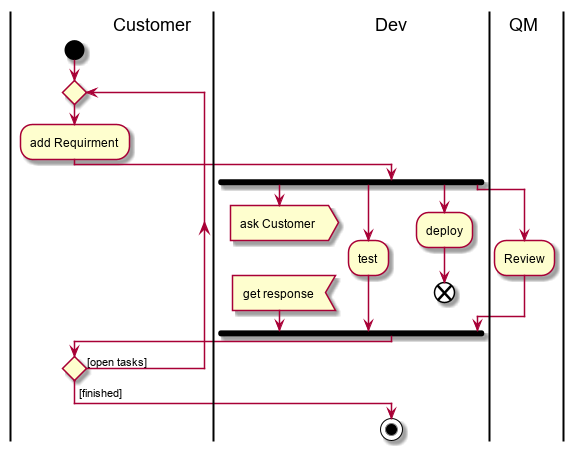
\includegraphics[width=5cm]{11_aufhuebschen01}
		}
	}
	Minimalbeispiel
	&
	
	\raisebox{-\height}{
		\href{https://www.planttext.com/?text=ZLB1Ri8m33sJhx0umM4_01DYKEt4a0QxJ8Y3rPWsQffaYKk5W7zVMc03jadBnScpt_Dpad5Wz5oLMeH26OSUIqXeWvNcPsjuZYL1TrQbIY8iqGHuspcglMBoNN75UKfPRHNlzWBYcc1QPDvMHawjjXw2iVKfORqaVm8JzCLI8zD4LzHc4uMbDVAUdUKsS9t7dZTLVqg9uvMnkMNQ_wFtVTEPod9-9wsZy-FDfDxR-dULmxGAR4loX-QGqBQDho-7-rnxwJ5wSeJDPe1Ime8-AkLBCZoyuc-iBrg70mm5N5H6efCGOvgBpY0ZZah1MHFeySm0p50PQAIPGYlu3JUe9AVjhi79o1-ai-bOjw2jelfSzsNcPXgu30BnaJH1hmygG6zb7HdWw3gi--9XjDeeeq9ESZqKf-6YX0CnZiBD1_m4}{
		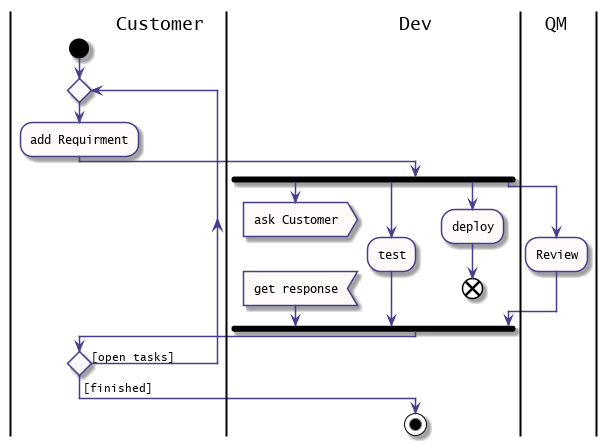
\includegraphics[width=5cm]{11_aufhuebschen02}
		}
	}
	Anpassung von Schriftart und Farben
	& 
	\raisebox{-\height}{
		\href{https://www.planttext.com/?text=PL3D3i8W63lBKtn7T_05d35BzEh1NHSFHAeZRe1yJ6EoXnVc_3yLIjkq51oa3rtR2A9-rN6mBNoVBcjS1jnk-j-tmHFHmq6cmrmgHINEdVOjJCW__0VhJn6IXa_qJ5cAoHf1xcincHyHOX8xQnYBqK7oABMX51t0G-2RJgo2Q-mjyJ3gppIMZheI5uthg7kL-Lf3po5qhNK3ccQacQQLTJ0KOclUPMAsh0xQQAwXThbuZ8iHZaGHWzF_tG40}{
		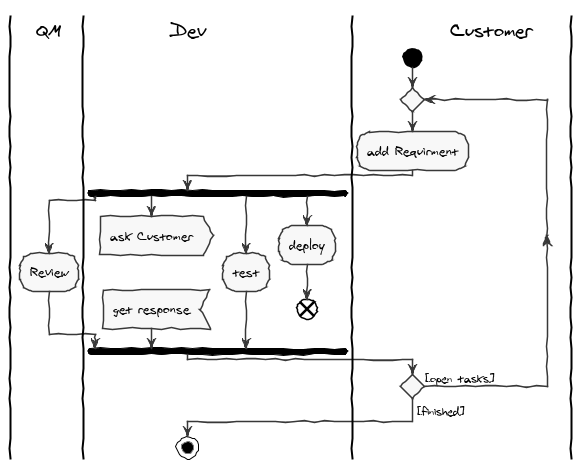
\includegraphics[width=5cm]{11_aufhuebschen03}
		}
	} 
	
	Sieht nach Entwurf aus: um die Vorläufigkeit und Änderbarkeit zu unterstreichen kann man es nach einer Skizze aussehen lassen.
	\\
	
	\begin{lstlisting}[style=plantuml]
@startuml
|Customer|
|Dev|
|QM|
|Customer|
start
repeat
:add Requirment;
|Dev|
fork
:ask Customer>
Detach
:get response<
fork again 
:test;
fork again
:deploy;
end
fork again 
|QM|
:Review;
end fork
|Customer|
repeat while () is ([open tasks])
->[finished];
|Dev|
stop 
@enduml
	
	\end{lstlisting}
	&
	\begin{lstlisting}[style=plantuml]
@startuml
skinparam DefaultFontName "Lucida Sans Typewriter"

skinparam Activity{
BackgroundColor snow
BorderColor DarkSlateBlue
DiamondBackgroundColor ghostwhite
DiamondBorderColor DarkSlateBlue

}
skinparam Note{
BorderColor DarkSlateBlue
BackgroundColor LightYellow
}

skinparam ArrowColor DarkSlateBlue
|Customer|
|Dev|
|QM|
|Customer|
start
...
stop 
@enduml
	\end{lstlisting}
	
	&
	
	
	\begin{lstlisting}[style=plantuml]
@startuml
' Welche Schriften gibt es auf dem System?
' listfonts als plantUML-Kommando gibt's aus.
skinparam DefaultFontName "FG Virgil"
skinparam handwritten true
skinparam monochrome true
skinparam packageStyle rect
skinparam shadowing false


|Customer|
|Dev|
|QM|
|Customer|
start
...
stop 
@enduml
	\end{lstlisting}
	
\end{tabular}

\begin{thebibliography}{9}
	\bibitem[plantUML]{plantUML}{Projektwebsite.},
	Dokumentation \\
	\url{	https://www.plantuml.com/}
	\bibitem[plantText]{planttext}{Projektwebsite.},
	Website, auf der direkt plantUML-QUelltexte geparst werden können: \\\url{https://www.planttext.com/}
\end{thebibliography}





\end{document}
